In Abbildung \ref{fig:dirac_flow_general} ist das Prinzip des DirAC Algorithmus zu sehen. Die $M$ Mikrofonkanäle werden mittels STFT (oder Filterbank) in den Frequenzbereich gebracht. Es wird ein Pseudointensitätsvektor gebildet (ähnlich dem $r_e$-Vektormodell aus \cite{ambi-book}), der im Analyseschritt verwendet wird, um die Diffusität $\Psi$ und Schalleinfallsrichtung $D$ pro Frequenzband des Signals zu ermitteln. Hier fließt die resultierende psychoakustische Annahme ein (siehe \ref{annahmen}), weswegen nur eine Richtung pro Frequenzband ermittelt wird.

\begin{figure}[!ht]
  \centering
  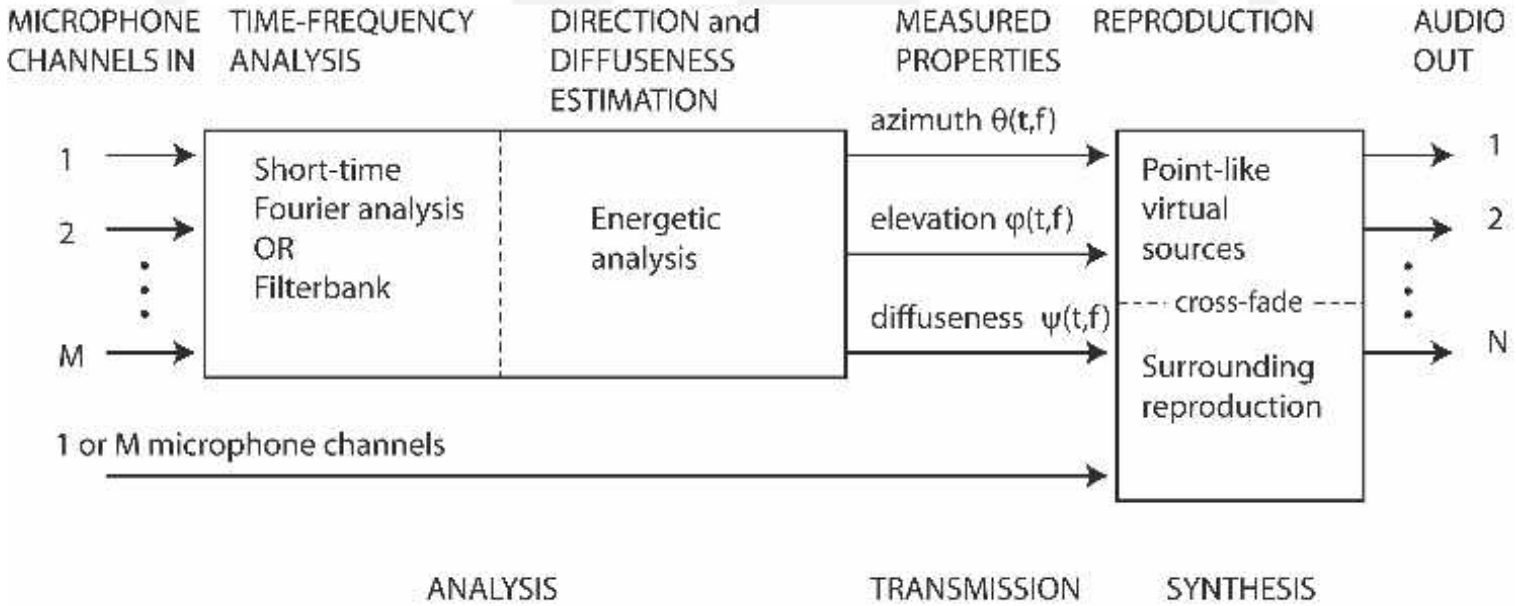
\includegraphics[width=0.9\textwidth]{funktionsweise/pic/pulkki_dirac_flow.png}
  \caption{Prinzip des DirAC Algorithmus\protect\footnotemark}
  \label{fig:dirac_flow_general}
\end{figure}

\footnotetext{Quelle: \cite{pulkki}}

Aus den $M$ Eingangskanälen werden mit virtuellen Mikrofonen die $N$ Ausgangskanäle gebildet (siehe Abbildung \ref{fig:dirac_flow_high}). Mit den ermittelten Eigenschaften werden die $N$ Kanäle spektral in einen gerichteten Anteil und in einen Diffusanteil getrennt. Der gerichtete Anteil hat bereits eine höhere Auflösung als die Eingangskanäle. Der Diffusanteil wird mit einem Dekorrelationsverfahren zur Erhöhung der Diffusität bearbeitet (siehe \ref{dekorrelation}). Anschließend werden die beiden Signalanteile per Addition wieder zusammengebracht und via iSTFT wieder in den Zeitbereich transformiert.

\begin{figure}[!ht]
  \centering
  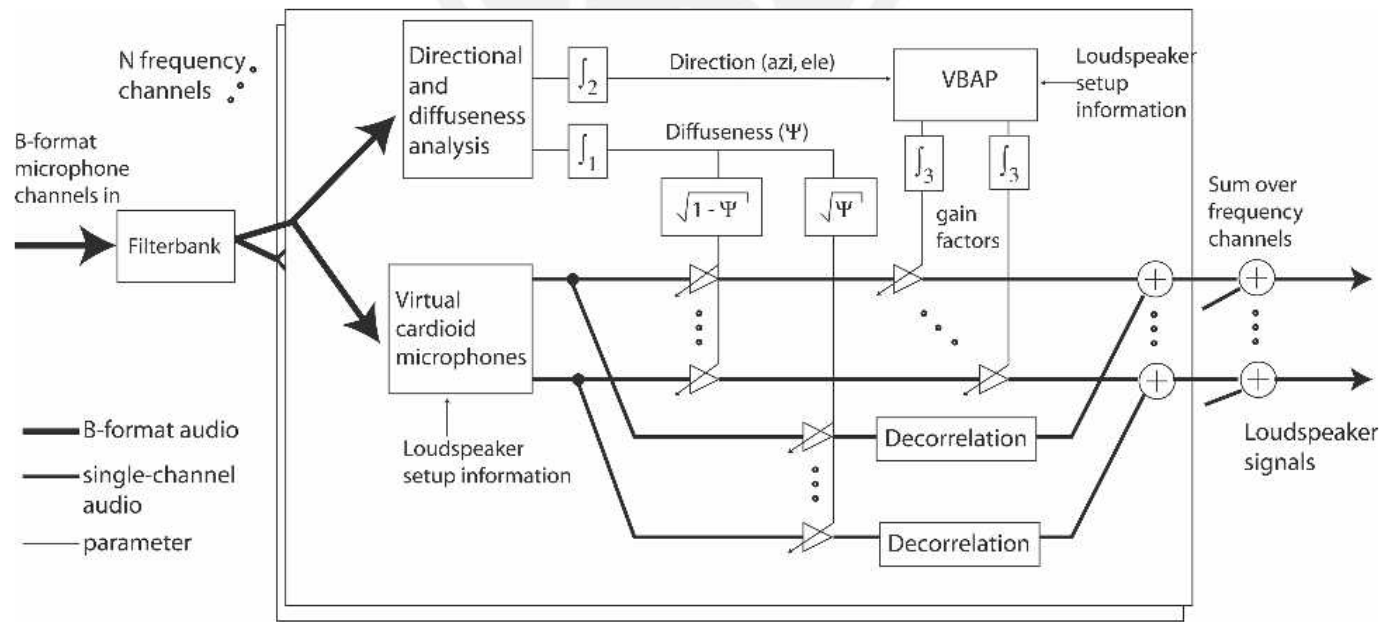
\includegraphics[width=0.9\textwidth]{funktionsweise/pic/pulkki_dirac_flow_2.png}
  \caption{DirAC zur hochqualitativen Reproduktion von B-Format Signalen\protect\footnotemark}
  \label{fig:dirac_flow_high}
\end{figure}

\footnotetext{Quelle: \cite{pulkki}}

In dieser Seminararbeit (und dem Hörversuch) wird ausschließlich diese Variante des DirAC-Algorithmus verwendet, der für eine hohe Audioqualität entwickelt wurde. In Abbildung \ref{fig:dirac_flow_low} ist eine andere Variante abgebildet, bei der die Signalübertragung eine größere Rolle spielt. Die Integralzeichen in den Abbildungen symbolisieren eine zeitliche Mittelung der Parameter zur Vermeidung von Artefakten.

\begin{figure}[!ht]
  \centering
  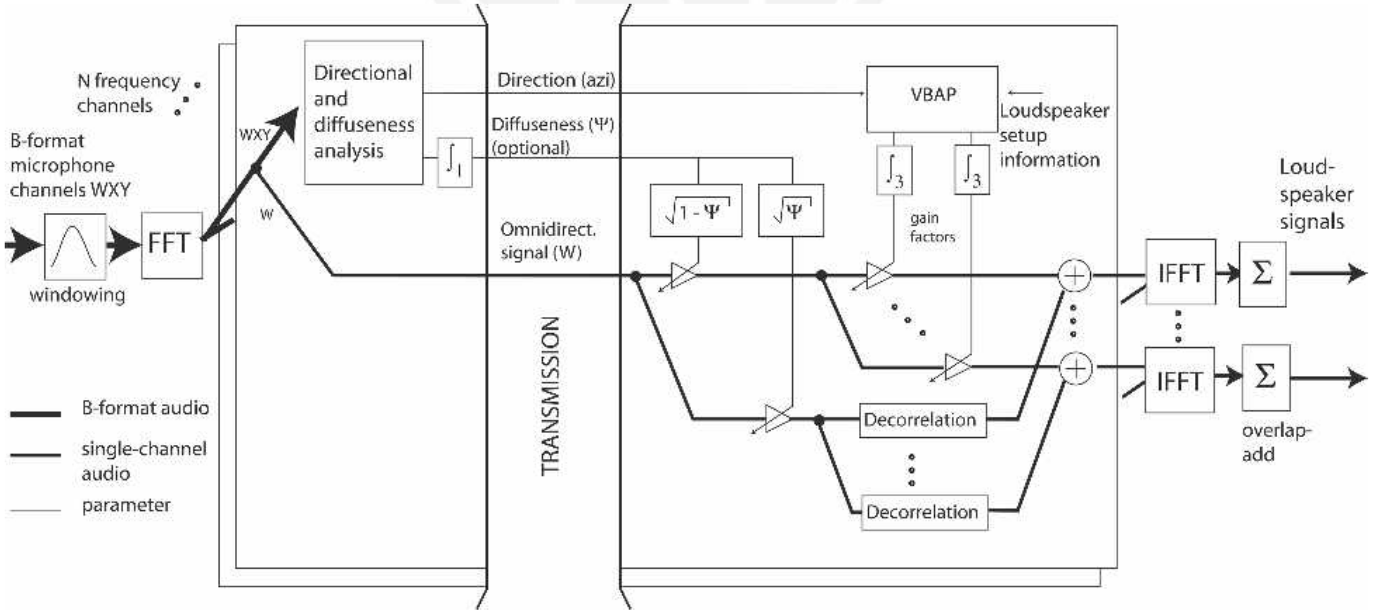
\includegraphics[width=0.9\textwidth]{funktionsweise/pic/pulkki_dirac_flow_3.png}
  \caption{DirAC für Telekommunikation\protect\footnotemark}
  \label{fig:dirac_flow_low}
\end{figure}

\footnotetext{Quelle: \cite{pulkki}}
